\documentclass{article}
\usepackage[utf8]{inputenc}
\usepackage[T1]{fontenc} 
\usepackage[french]{babel}
\usepackage{graphicx}
\usepackage{subcaption}
\usepackage[table]{xcolor}
\usepackage{longtable}
\usepackage{geometry}
\usepackage{hyperref}
\usepackage{appendix}
\usepackage{pdfpages}

\geometry{hmargin=2.5cm,vmargin=3cm}
\setlength{\parskip}{0.15cm}

\title{Rapport de Stage}
\author{Laureline MARTIN}
\date{Mercredi 7 Octobre 2020}

\begin{document}
\maketitle
\vspace*{14cm}
\begin{center}
	\textbf{Encadrants :}
\end{center}
\begin{tabular}{p{4cm}p{4cm}p{8cm}}
	\hspace*{-1cm}
	Mme. Viviane GAL & Ingénieure & Equipe \textit{Interactivité pour lire et jouer - ILJ}\smallskip\\
	\hspace*{-1cm}
	M. Eric GRESSIER-SOUDAN & Professeur des universités & Equipe \textit{Réseaux et Objets Connectés - ROC}
	\smallskip\\
	\hspace*{-1cm}
	Mme. Elena KORNYSHOVA & Maître de conférences & Equipe \textit{Igénieurie des systèmes d'information et de décision - ISID}
\end{tabular}

\newpage
\begin{center}
	\textbf{Résumé :}
\end{center}
\hspace*{0.4cm}
Durant cinq mois et demi, j'ai travaillé au laboratoire de recherche CEDRIC au Conservatoire National des Arts et Métiers de Paris.\par
Ce stage s'est inscrit au sein du projet exploratoire "Conception et développement des jeux pervasifs adaptables avec la prise en compte des états émotionnels des joueurs" du laboratoire.
L'objectif global de ce projet est de proposer un jeu pervasif où le joueur et ses émotions sont au coeur même du jeu. 
Pour cela, des capteurs physiologiques sont utilisés pour détecter et reconnaître les états émotionnels du joueurs ainsi que des capteurs placés dans l'environnement pour connaître le contexte global. 
Ces capteurs génèrent beaucoup de données qu'il faut traiter en temps-réel pour une adaptation dynamique du jeu.
Dans ce rapport, nous prposons une solution pouvant ingérer les données provenant de capteurs physiologiques en temps-réel.
Ensuite, cette solution envoie ces données à des algorithmes déjà existant qui permettent de déduire des états émotionnels.
Un état de l'art ainsi qu'une première version d'une ontologie afin de répondre à cet objectif ont été proposées et se trouvent dans ce rapport. 
\bigskip\newline
\begin{center}
	\textbf{Abstract :}
\end{center}
\hspace*{0.4cm}
I worked for the CEDRIC research laboratory based on Conservatoire Nationnal des Arts et Métiers at Paris during five mounths and half.\par
This work was for the laboratory's exploratory project "Desing and development of adaptables pervasives games to players' emotional states".
The main project goal is to develop a pervasive game where player and his emotions are the heart of the game.
To reach this goal, physiological sensors are used in order to detect and recognize player's emotional states and others sensors are placed in environment to know the global context.
Sensors generate a lot of data that must be processed in real-time to a dynamic game's adaptation.
This report contains a solution to ingest real-time physiological sensors' data.
This solution sends data to existing detection and recognition of emotional states algorithms.
This report contains a state of the art and a first version of an ontology that I made too. 
%\vspace*{3.1cm}
\vfill
\begin{center}
	\textbf{Avant-propos}
\end{center}
\hspace*{0.4cm}
Dans le cadre de la validation du Master 2 Data Managment in a Digital World - Datascale, proposé par l'Université de Versailles Saint-Quentin / Paris Saclay, j'ai effectué un stage de cinq mois et demi du 16 Mars 2020 au 30 Septembre 2020.
Le contexte particulier lié à la crise sanitaire m'a amené à travailler pour la majorité de mon stage en télétravail (du 16 Mars au 10 Septembre).\par
Pour communiquer pendant cette période de travail à distance, nous utilisions les mails et nous avons organisé des réunions via Teams tous les 7 à 15 jours.
Ces réunions duraient entre une demie heure et une heure.
Ces sessions vidéos étaient l'occasion de faire le point sur l'avancement de mon travail et sur les tâches des jours à venir.
Cependant, la barrière de l'écran a créé un réel manque de spontanéité lors de nos échanges.
Pour ma part, je pense que les visio-conférences n'ont pas suffit pour échanger tout au long de cette période de télétravail. 
Peut-être qu'une autre forme de communication, comme une messagerie instantanée, ajoutée à celle des réunions sur Teams, aurait pu réduire se manque de spontanéité.\par
A l'issue de ce stage, je pense que les réunions en présentiel restent la meilleure manière de communiquer et de partager autour d'un projet.

\newpage
\renewcommand{\contentsname}{Table des matières}\tableofcontents

\newpage
\section{Introduction}
	Depuis plusieurs années, les jeux pervasifs se multiplient sur le marché, proposant aux joueurs des contenus très immersifs.
	Le jeu pervasif (aussi appelé jeu omniprésent) est un genre de jeu qui mêle le monde physique et le monde numérique et rend floue cette frontière.
	Dans le jeu pervasif, le contexte est essentiel. 
	Comme le montre \cite{astic_2013}, quatre facteurs sont mis en jeu : l'espace, le temps, la technologie et les rapports sociaux. 
	L'espace du jeu pervasif est à la fois ancré dans le réel et dans le virtuel.
	Il convient alors que des ponts existent entre ces deux espaces. 
	Ces ponts peuvent se faire via des objets, des points géographiques, des personnes, etc. 
	Le temps est calqué sur le temps réel mais il peut être utilisé de différentes manières dans le jeu. 
	Par exemple, l'heure et/ou le jour peuvent influencer le comportement que doit adopter le joueur.
	La technologie est également importante. 
	Elle doit rester accessible au joueur, tant sur le plan pratique que sur le plan financier. 
	La géolocalisation, les réseaux sans fil, etc. sont des technologies utilisées pour ce type de jeu.
	Dans les jeux pervasifs, les joueurs, les spectateurs et les non-joueurs sont mélangés sur le même espace. 
	Les joueurs n'ont pas de caractéristiques particulières pour se reconnaître.%\par
	Le jeu pervasif à un un impact social et culturel important.
	Il favorise les récontres dans l'espace physique.
	Il permet de découvrir de nouveaux endroits, de nouvelles choses et de s'enrichir culturellement.
	Cependant, le jeu omniprésent ne met pas réellement le joueur au centre de jeu.\par
	Le projet "Conception et développement des jeux pervasifs adaptables avec la prise en compte des états émotionnels des joueurs" vise à mettre le joueur et ces émotions au centre du jeu.
	Ce seront les émotions du joueurs qui influenceront le jeu et ses événements.\par
	Pour pouvoir détecter et reconnaître les états émotionnels du joueur afin que le jeu s'y adapte et propose l'événement le plus adéquat, de multiples capteurs physiologiques peuvent être utilisés.
	Ces capteurs génèrent beaucoup de données qui doivent être stockées et traitées.
	Ces données permettront à des algorithmes de reconnaître les états émotionnels.\par
	Le but de ce travail a été de dresser le contour d'un jeu pervasif adaptable aux états émotionnels du joueur et d'en affiner la conceptualisation.
	Dans ce rapport, nous nous sommes intéressés, d'une part, à l'adaptation de jeux selon le contexte émotionnel et d'autre part, à la gestion de données générées par des capteurs physiologiques.\par
	Dans un premier temps, nous présenterons dans la Section \ref{sec:cedric} le laboratoire CEDRIC.
	Puis, dans la Section \ref{sec:projet}, nous parlerons du projet, des ses objectifs et de la problématique nous traiterons dans ce rapport.
	nous décrirons, dans la Section \ref{sec:etatart}, notre état de l'art comparant différentes approches pour l'adaptation dynamique d'un jeu pervasif aux états émotionnels du joueur. 
	Nous aborderons dans la Section \ref{sec:escape} l'expérience que nous avons menée lors d'un escape game et la notion d'expérience utilisateur.
	Dans la Section \ref{sec:modelisation}, nous présenterons une ontologie en cours de construction d'un jeu pervasif prenant en compte l'état émotionnel du joueur et le bilan que nous tirons de cet exercice.
	Enfin, nous expliquerons dans la Section \ref{sec:prototypage} une solution que nous avons conçue pour la gestion de données en temps-réel provenant de capteurs physiologiques.

\section{Présentation du laboratoire CEDRIC}\label{sec:cedric}
	\begin{center}
		
\includegraphics[scale=0.55]{../include/logo-cedric.PNG}\\
	\end{center}\par
	Avant de présenter le travail réalisé, nous allons faire une présentation du laboratoire CEDRIC.
	Le laboratoire de Centre d'Etudes et De Recherche en Informatique et Communication (CEDRIC)\footnote{\href{http://cedric.cnam.fr/lab/accueil/labo/}{http://cedric.cnam.fr/lab/accueil/labo/}} au sein du Conservatoire National des Arts et Métiers (CNAM) de Paris\footnote{\href{http://www.cnam.fr/portail/accueil-conservatoire-national-des-arts-et-metiers-821166.kjsp}{http://www.cnam.fr/portail/accueil-conservatoire-national-des-arts-et-metiers-821166.kjsp}}. 
	Le laboratoire se situe au 2 rue Conte 75003 PARIS.\par
	Le laboratoire CEDRIC est composé de huit équipes menant des recherches et des actions dans le domaine de l'informatique fondamentale et appliquée, ainsi que dans d'autres disciplines proches telles que les statistiques, électronique,....\par
	Les équipes du laboratoire sont les suivantes :
	\begin{itemize}
		\item L'équipe Données complexes, apprentissage et représentations (Vertigo) : Extraire de l'information et construire des méthodes de gestion de données basées sur le contenu pour des données massives audios, images et vidéos;
		\item L'équipe Interactivité pour Lire et Jouer (ILJ) : Questions autour de l'interaction Homme-Machine concernant des activités telles que le jeu et la lecteure. Cette équipe mèle plusieurs disciplines (l'informatiques, la psychologie, le design, les arts,...) afin de répondre aux études en cours qui concernent la modélisation de la difficulté dans les jeux, les méthodologies de game design inclusif, etc.;
		\item L'équipe Ingénieries des Systèmes d'Information et de Décision (ISID) : Cette équipe s'est réunie autour de trois axes de recherche : les systèmes décisionnels, le web sémantique et la qualité des systèmes d'information. Son but est de concevoir des méthodes, des outils et des techniques	pour la conception et l'analyse de systèmes d'information et de décision dans tous les domaines;
		\item L'équipe Traitement du signal et architectures électroniques (LAETITIA) : Concentrée sur trois axes de recherhe : le traitement du signal pour les télécommunications (recherches en lien avec les réseaux cellulaires (5G/6G) et en lien avec les problématiques de couches physique pour les réseaux faible puissance longue portée pour l'IoT), la sûreté de fonctionnement des sytèmes dynémiques (recherche en automatique) et l'implémentation temps-réel (mise en oeuvre des algorithmes proposés par l'équipe);
		\item L'équipe Méthode Statistique de Data-Mining et Apprentissage (MSDMA) : Traitement de données et développement de modèles d'apprentissage statistiques dans le but d'extraire des informations pour prise de décision;
		\item L'équipe Optimisation Combinatoire (OC) : Rassemblée autour de deux axes : la programmation mathématique et applications ainsi que les graphes et optimisation;
		\item L'équipe Réseaux et Objets Connectés (ROC) : Porte sur l'analyse et l'exploitation des nouvelles architectures réseaux et des systèmes liés à la virtualisation, à la mobilité et au développemnt des objets connectés;
		\item L'équipe Systèmes Sûrs (SYS) : Spécialisation, conception, vérification et évaluation des systèmes. Pour cela, Les recherches se font autour de trois axes : l'axe typage, sémantique et preuve, l'axe architecture logiciel, architecture systèmes et ligne de produit et l'axe vérification et évaluation de systèmes parallèles et asynchrones.
	\end{itemize}

\section{Cadre du projet}\label{sec:projet}
	Le projet exploratoire intitulé "Conception et développement des jeux pervasifs adaptables avec la prise en compte des états émotionnels des joueurs" a éé initié par trois enseignants-chercheurs du laboratoire CEDRIC du CNAM de Paris.
	Il s'agit de Mme. Viviane GAL (équipe ILJ), M. Eric GRESSIER-SOUDAN (équipe ROC) et Mme. Elena KORNYSHOVA (équipe ISID).
	Ce projet vise à élaborer un jeu pervasif capable de s'adapter dynamiquement selon le contexte du joueur et au contexte de son environnement.\par
	Dans cette section, nous allons présenter l'objectif global de ce projet.
	Puis, nous parlerons de la problématique à laquelle nous apporterons une solution.
	Nous donnerons aussi des définitions essentielles pour les notions clés et nous aborderons les sujets connexes que nous verrons tout au long de ce rapport.
	\subsection{Motivations et objectif du projet}\label{sec:objectif}
		Avec le jeu pervasif, il est possible de créer une grande immersion et une plus grande implication (i.e. engagement) du joueur pour le jeu en comparaison à d'autres types de jeux tels que les jeux vidéos ou les jeux de sociétés.
		L'idée principale de notre projet est de concevoir un jeu omniprésent capable de détecter et de reconnaître dynamiquement l'état émotionnel courant de joueur. 
		Le jeu devra aussi être capable de s'adapter à cet état en temps-réel en proposant un événement spécifique. 
		La Figure \ref{fig:motivation} schématise l'objectif de notre projet.
		\begin{figure}
			\centering
			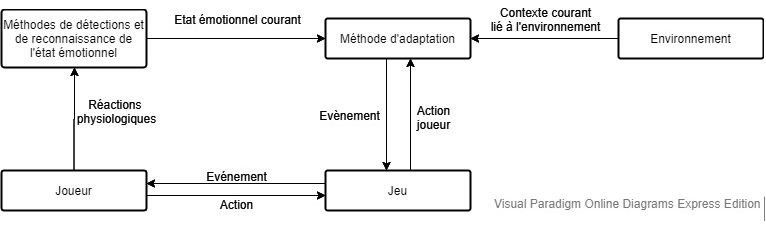
\includegraphics[scale=0.75]{../include/motivation.jpg}
			\caption{Objectif global du projet}
			\label{fig:motivation}
		\end{figure}
		Un joueur qui jouera à notre jeu aura une ou des réaction(s) physiologique(s) qui traduiront un état émotionnel détecté et reconnu par nos algorithmes.
		Cet état émotionnel courant sera indiqué à nos algorithmes d'adaptations qui receveront aussi des indications sur l'état courant de l'environnement et sur les actions que fait le joueur dans le jeu.
		Les algorithmes d'adaptation indiqueront au moteur de jeu l'événement le plus indiqué.
		Et le jeu affichera cet événement sur l'interface utilisateur, ce qui enclenchera de nouvelles réactions physiologique, etc.\par
		La réponse adaptatée du jeu à l'état émotionnel de son joueur devra se faire sous la forme d'événments dans le jeu.
		Les événemnts particularisés à l'état émotionnel du joueur devront soit :
		\begin{itemize}
			\item Avoir tendance à provoquer le même état émotionnel que celui expérimenté par le joueur à cet instant afin de le maintenir dans cet état émotionnel;
			\item Avoir tendance à provoquer un autre état émotionnel que celui expérimenté par le joueur à cet instant dans le but de provoquer un changement d'état émotionnel.
		\end{itemize}
		Le choix d'utiliser un événement plutôt qu'un autre afin d'essayer d'influencer l'état émotionnel du joueur devra se faire selon différents critères.
		Ces critères pourraient être : la valeur positive/négative de l'état émotionnel (même si la réalité est bien plus complexe), l'avancement dans le jeu, ou bien le contexte environnemental courant.
		Bien sûr, d'autres critères sont envisageables.
		Le but d'une telle adaptation est de pouvoir garantir l'expérience de jeu la plus immersive possible et un meilleur divertissement pour le joueur.\par
		Toutefois, la conception d'un tel jeu devra rester assez générique.
		L'une de nos motivations finales est de pouvoir appliquer notre jeu à d'autres domaines dans de prochains projets.
		D'autres domaines d'applications pourraient être le domaine du médicale ou celui de l'apprentissage.
	\subsection{Problématique}\label{sec:problematique}
		Pour un projet aussi vaste qu'est le nôtre, plusieurs problématiques se posent.
		Par exemple, nous pouvons nous intéresser aux moyens de détecter et de reconnaître les états émotionnels d'une personne.
		Nous pourrions aussi nous intéresser aux problématiques liées à l'adaptaion du jeu pervasif.
		Les méthodes et les règles qu'il faudrait utiliser pour une "bonne" adaptation du jeu pervasif à son joueur sont à définir.\par
		La problématique à laquelle nous avions tout d'abord tenté d'apporter une contribution était celle de la réalisation d'un modèle conceptuel pour représenter l'adaptation d'un jeu pervasif aux émotions d'un joueur.
		Mais, au cours de notre travail, nous avons décidé de changer de point de vue et  d'aborder une autre problématique également importante pour l'aboutissement de notre projet.\par
		Dans ce rapport, nous allons traiter principalement la problématique de la gestion des données générées par les capteurs physiologiques.
		Pour atteindre notre objectif final, il est important de pouvoir utiliser les données des capteurs pour déterminer les états émotionnels afin que le jeu puisse s'y adapter. 
		Cela pose une contrainte importante sur la gestion des données en temps-réel.
		En effet, la réponse adaptée à l'état émotionnel courant du joueur doit être la plus immédiate possible afin de ne pas créer un sentiment de décalage entre le ressenti du joueur et l'adaptation du jeu.
	\subsection{Définitions et sujets connexes}\label{sec:connexe}
		Avant de développer les travaux que nous avons menés, il est important de faire une mise au point sur les termes que nous allons employer tout au long du rapport.\par
		Ici, nous parlons d'état émotionnel et non d'émotion.
		L'émotion est une réaction physiologique forte qui ne dure que quelques minutes.
		Elle est la réponse à un événement, à un stimuli,...
		L'ensemble des émotions est très restreint.
		Il se composent, selon les définitions de quatre à huits émotions.
		L'état émotionnel, quant à lui, est plus vaste. 
		Il regroupe plusieurs notions en plus de l'émotion telles que le sentiment ou l'affect. 
		L'état émotionnel est donc une définition "étendue" de l'émotion, ce qui nous permet de ne pas exclure des notions que nous pourrions considérer dans de futurs travaux.
		Cela nous permet aussi de rester assez vaste sur les possibilité de reconnaissance de notre jeu.\par
		Pour répondre à la problématique de la gestion de données en temps-réel provenant de capteurs physiologiques, nous avons besoin d'avantage de contexte sur des sujets tels que : les méthodes de détections et de reconnaîssance des états émotionnels, la notion d'expérience utilisateur et d'autres types de jeux.
		Tout au long du rapport, nous allons aborder ces sujets qui n'entre pas directemnt dans le cadre de la solution que nous apportons mais qui sont essentiels pour la compréhension du sujet de notre projet et de l'apport de notre solution.

\section{Etat de l'art}\label{sec:etatart}
	Notre état de l'art s'intéresse aux différentes méthodes déjà existantes dans la littérature scientifique et technique permettant à différents types de jeux de s'adapter aux états émotionnel de leurs joueurs.\par
	Dans l'état de l'art, nous proposons un cadre que nous avons conçu pour comparer des approches pour l'adaptation de jeux aux états émotionnels des joueurs. Le cadre s'appuie sur les critères suivants :
	\begin{itemize}
		\item Les méthodes pour la détection et pour la reconnaissance des états émotionnels
		\begin{itemize}
			\item Les capteurs utilisés
			\item Les algorithmes utlisés pour la détection et/ou la méthode de l'état émotionnel
		\end{itemize}
		\item Les autres caractéristiques de l'utilisateur prises en compte par le jeu
		\item Les méthodes d'adaptation d'un jeu au contexte de son utilisaeur
		\begin{itemize}
			\item Méthodes pour l'adaptation du jeu selon l'état émotionnel du joueur
			\item Méthodes pour l'adaptation du jeu selon d'autres caractéristiques du joueur
		\end{itemize}
	\end{itemize}
	L'état de l'art se trouve en Annexe \ref{ann:eda}.\par
	Ce cadre nous permet de répérer par exemles les algorithmes communs ou divergeant utilisés pour la reconnaissance d'états émotionnels ou bien de comparer les états émotionnels évalués par chaque méthode.\par
	De cette comparaison, il en ressort plusieurs questions et limites.
	Tout d'abord, on remarque que seulement quelques états émotionnels sont traités dans les approches. 
	Même si on peut imaginer que certains états émotionnels ne seront jamais expérimentés au cours du jeu que nous souhaitons concevoir, il semble tout de même important de pouvoir prendre en compte le plus grand nombre d'états émotionnels possible.
	Sans quoi, le jeu pourrait mal s'adapter au joueur et impacter négativement son niveau d'intérêt pour le jeu.\par
	Dans notre cas, nous utilisons des capteurs physiologiques de contact, c'est-à-dire des capteurs "collés" au joueur, dans le but d'acquérir des données sur son état physiologique pour en déduire son état émotionnel courant via des algorithmes.
	Dans les approches que nous avons relevés, certaines d'entre elles reconnaissent des états émotionnels en utilisants différents types d'algorithmes et des capteurs physiologiques. 
	Mais contrairement à cela, d'autres utilisent des modèles pour "prédire" l'état émotionnel courant du joueur.
	Ce genre de méthodes "prédictives" peuvent être intéressantes car elle retire l'équipement de capteurs du joueur.
	Cependant, ce type de méthodes semble être moins précis car il se base sur le principe que tous les joueurs ressentiront exactement le même état émotionnel lorsqu'ils se retrouveront dans le même cas de figure.
	De plus, cela implique d'envisager absolument tous les états du jeu possibles, toutes les actions possibles et d'associer un état émotionnel pou chacque intersection.
	Ce qui nous fait croire que l'utilisation de capteurs physiologiques, même si leur utilisation est plus contraignante pour le joueur, est plus pertinente car plus proche de chacun.
	Nous pensons que deux états émotionnels pourront être expérimentés par deux joueurs différents, même s'il s'agit de la même situation dans le jeu pour les deux joueurs.
	De ce fait, il est nécessaire que le jeu s'adapte à chacun dynamiquement.\par
	Notre cadre de comparaison révèle que d'autres caractéristiques que celle de l'état émotionnel peuvent être considérés pour augmenter la connaissance du sur son joueur.
	Ces caractéristiques peuvent être intéressantes à étudier à la fois pour la détection et la reconnaissance de l'état émotionnel mais aussi pour l'enrichissement de la connaissance du contexte de l'environnement globale. 
	Ces caractéristiques peuvent aussi bien s'appuyer sur un questionnaire de préférence rempli par l'utilisateur lui-même que sur la présence de capteurs dans l'environnement.\par
	Cet état de l'art, nous a permis d'avoir une vision de ce qui existait déjà en matière d'adaptation de jeux aux états émotionnels des joueurs.
	Il aura aussi été l'occasion de proposer un cadre de comparaison pour ce sujet.
	Grâce à cet état de l'art, j'ai pu comprendre quels sont les enjeux pour la réalisation de notre objectif.

\section{Expérience d'un Escapte Game}\label{sec:escape}
	Nous avons expérimenté sur nous-mêmes un escape game.
	La salle que nous avons testée se trouve au Victory Escape Game\footnote{\href{http://www.victoryescapegame.fr/}{http://www.victoryescapegame.fr/}} situé au 37 rue des Gravilliers à Paris.
	Cela a été l'occasion d'expérimenter ce genre de jeu très immersif.\par
	Dans cette section, nous allons tout d'abord aborder la notion d'expérience utilisateur.
	Puis nous ferons un retour sur cette expérience d'escape game et ce qu'elle a pu apporté sur le travail mené.
	\subsection{Expérience Utilisateur}\label{sec:UX}
		L’expérience utilisateur (UX pour User eXperience) concerne toutes les réactions qu’un utilisateur peut avoir lors d’une interaction avec un service, un objet, un espace public, etc.
		C’est aussi tout ce que l’utilisateur peut ressentir lors de cette interaction.
		L’expérience utilisateur va donc plus loin que la simple notion d’ergonomie qui elle ne concerne que la « facilité d’utilisation » d’un produit.\par
		L’UX commence par la perception sensorielle de l’utilisateur de ce qu’il lui est présenté. 
		Cette perception est « analysée » par le cerveau et mémorisée.
		Une réaction est ensuite faite.
		Les concepteurs peuvent alors analyser ces réactions et améliorer leur conception.
		Cette dernière étape est appelée UX Design.
		L’UX Design c’est éprouver un prototype par des utilisateurs de manière itérative.
		Après chaque test utilisateur, le prototype est amélioré et testé à nouveau par des utilisateurs.\par
		L’UX désigne un vaste champ d’application.
		Dès lors qu’une interaction se fait entre un utilisateur et quelque chose, on peut parler d’expérience utilisateur.
		De ce fait, de nombreuses définitions de l’UX existent.
		Chacune d’entre elles tend à s’appliquer d’avantage à un domaine qu’à un autre.
		Dans le cadre de nos recherches, nous traiterons ici uniquement de l’expérience utilisateur dans les jeux.\par
		Une « bonne » UX vise à maximiser d’une part l’utilisabilité d’un jeu et d’autre part l’engagement du joueur.\par
		L’utilisabilité rassemble toutes les questions qui concernent la facilité du jeu.
		Cela va de la visibilité et de la compréhension des affichages dans le jeu par le joueur à la facilité de faire des actions.
		Par exemple, la souris d’un ordinateur étant généralement à droite, on évitera de demander au joueur à la fois de cliquer sur la souris et d’appuyer sur des touches situées sur la droite du clavier.
		En UX design il existe des cadres et des règles à appliquer pour une bonne utilisabilité d’un jeu.\par
		L’engagement (i.e. le flow ou l’immersion) concerne la partie « émotionnelle » de l’interaction entre le joueur et le jeu.
		Il s’agit de réussir à motiver le joueur à commencer ou à continuer à jouer.
		Cela peut se faire par l’accomplissement d’objectifs pour obtenir des récompenses.
		La progression, la coopération, la compétition, etc. sont également des éléments motivants pour le joueur.
		Créer des émotions au joueur tout au long de sa partie permet également un meilleur engagement.
		De plus, il faut que la difficulté du jeu soit bien « réglée » pour que le joueur n’ai ni une sensation d’ennui ni envie de rejeter le jeu.
		Cela peut passer par exemple par l’apprentissage du jeu via des tutoriels.
	\subsection{Expérimentation d'un Escape Game}\label{sec:expescape}
		L'escape game que nous avons expérimenté se présentait sous la forme d'une mission d'une heure.
		Le but de cette mission était d'entrer dans un vaisseau désafecté pour emprunter un portail de téléportation.
		Celui-ci étant cassé, il fallait récupérer des indices dissimulés dans les pièces pour le redémarrer.\par
		Tout d'abord nous avons été sensibilisé à la mission qui nous attedait par le maître du jeu. 
		Il s'agitssait d'une réunion d'une vingtaine de minutes pour nous expliquer d'une part les règles mais aussi notre objectif.
		Cette sensibilisation est un premier contact indirect avec le jeu et me semble tout aussi importante que le jeu en lui même.
		C'est une méthode pour nous motiver à joueur et à être performant dans notre jeu.
		Un sentiment de compétition est aussi implicitement donné lorsque le maître du jeu nous a indiqué les meilleurs temps d'autres joueurs.\par
		Le principe de l'escape game est de fouiller les pièces pour trouver des indices pour débloquer des mécanismes et rejoindre la sortie.
		Les indices étaient de toutes sortes : écrits, lumineux, objets, boutons poussoirs, textiles, etc.
		Il pouvait aussi se trouver de faux indices.
		Les pièces ont été décorés, pour donner l'impression d'un vaisseau spacial.
		Le but est de donner la sensation la plus forte possible au joueur qu'il se trouve dans une "véritable" station spaciale.
		Pendant cette partie, si le maître du jeu -qui se trouvait dans une autre pièce et qui nous observait grâce à des caméras et des micros- pouvait nous donner des indices grâce à un écran.
		Un message nous donnant un indice sur le mécanisme à débloqué appariassait accompagné d'un indicateur sonore.
		Les messages que nous recevions par cet écran faisait penser qu'il s'agissait d'indications données par une intelligence artificelle.\par
		Tous les objets et le décor des différentes pièces permet de créer une ambiance et ploger immédiatement les joueurs dans l'univers où les créateurs du jeu essaye de les emmener.
		Nous avons pu également relever quelques méthodes d'UX design comme l'utilisation d'objectifs à attiendre.
		Par exemble, l'objectif principal est de sortir du vaisseau avant le temps imparti (une heure) et pour y parvenir, il faut réussir à ouvrir différentes portes pour accéder aux pièces suivantes.
		L'utilisation d'un compte-à-rebours affiché en permanance à l'écran créait un sentiment de stress.
		Chaque alerte sonore indiquant qu'un nouveau mécanisme avait été débloqué donné un sentiment de satisfaction.\par
		Nous n'avons pas réussi à arrivé jusqu'au bout de notre "mission". Cinq minutes avant la fin du compte-à-rebours nous sommes arrivés à la dernière salle.
		Nous nous attendions pas à cette dernière salle et avons été très surpris.
		Cela a été un peu frustrant de ne pas pouvoir terminer cette session avant la fin du compte-à-rebours.
	\subsection{Accessibilité d'un excape game}
		Dans cettte partie, je vais aborder les limites de l'accessibilité aux déficients visuels de l'ecape game et généraliser aux jeux. 
		Il s'agit d'un témoignage et non d'une recherche à part entière.
		Cette réflexion nous donnera une piste de réflexion pour notre propre jeu pervasif.\par
		Etant personnellement déficiente viuelle, je vais vous rapporter mon expérience personnelle de l'escape game que nous avons expérimenté.\par
		Pour atteindre l'objectif était de réparer portail de téléportation, il fallait rechercher dans différentes pièces des indices.
		Le premier obstacle rencontré lors cette partie était celui du déchiffrage des indices.
		En effet, beaucoup d'indices se base sur de l'écriture.
		Par exemple, nous avions trouvé un dossier contenant plusieurs pages écrites avec une taille de police standard (comme celle de ce rapport par exemple).
		Cet indice m'était donc inacessible, je distinguais seulement quelques logos qui se trouvais dans ce dossier.
		Un autre élément inacessible pour moi était une grande carte affiché dans une des pièce où il fallait retrouver des coordonnées et ajuster des boutons par rapport à ces coordonnées.
		Ce type d'élément m'était complètement inacessible car il s'appuie uniquement sur la capacité du joueur à repérer des éléments visuels parmis un tas d'informations visuelles entremélées.
		J'ai aussi rencontré des difficultés dû à la luminosité basse des pièces.
		De plus, avec la situation sanitaire actuelle, nous étions obligé de porter des gants pour jouer puisqu'il fallait toucher et prendre beaucoup d'objets.
		Cependant, porté des gants empêche de sentir beaucoup de chose et m'a privé d'informations par le touché que d'autres ont par le visuel.\par
		Toutes ces limites m'ont fait sortir du jeu et casser le rythme et l'intrigue.
		De ce point de vue là, je peux dire que mon expérience utilisateur à été moyenne.
		J'ai été "déconnecté" de certains indices et j'ai dû laissé mes coéquipiés prendre le relai sur ce que ne je pouvais pas voir.
		Ce qui a probablement joué sur leur expérience utilisateur également.
	\subsection{Bilan}
		Nous retenons plusieurs points de cette expérimentation.
		Cet escape game nous a permis d'appliquer à nous-même le ressenti de joueurs.
		Cela nous a permis de rappeler ce qu'était l'expérience utilisateur et à quoi cela pouvait servir pour améliorer un jeu.
		Nous avons pu expérimenter différentes états émotionnels lors de cette session.
		Le fait d'avoir ressenti différents états émotionnels et d'avoir été motivés durant toutes la partie à jouer montre que l'UX design est important pour le joueur, pour son expérience de jeu et pour son amusement.\par
		Cette expérience d'escape game et mon expérience personnelle m'a fait comprendre l'importance de mener des expérimentation "en réel".
		Bien souvent, les expériences sont menées en laboratoire.
		Comme celles décritent dans l'état de l'art (Annexe \ref{ann:eda}) ou celles menées pour amélioré l'UX.
		Nous remarquons que bine souvent, ces expériences n'impliquent que des personnes n'ayant aucun problème de santé, dans une fourchette d'âge restreinte, etc.
		Cette méthode d'expéiences exclus certains joueur et crée un décalage entre les testeurs du jeu et le public réel.
		D'après toutes ces remarques, il me semble important d'ouvrir le groupe test au public le plus large possible.
		Autrement dit, d'étendre les âges, les cultures, les capacités physiques, etc. le plus possible afin de permettre une plus grande inclusivité.

\section{Modélisation conceptuelle}\label{sec:modelisation}
	Dans cette partie, nous allons présenter un modèle conceptuel qui n'a pas pu être terminé. 
	Le but de ce modèle conceptuel était de réprésenter chaque composant permettant la prise en compte des états émotionnels dans le jeu pervasif et de s'y adapter. 
	Il fallait à la fois représenter le joueur, le jeu, les états émotionnels, les capteurs mais aussi des composants plus abstraits comme les réactions physiologiques du joueur, la reconnaissance des états émotionnels, l'adaptation dynamique du jeu, etc. 
	Ce modèle devait être représenté sous la forme d'une ontologie en utilisant le format standard du diagramme de classes UML.
	\subsection{Ontologie}\label{sec:ontologie}
		Le diagramme de la Figure \ref{fig:modele} représente notre modélisation pour les différents éléments qui composent un jeu pervasif adaptable aux états émotionnels du joueur. 
		\begin{figure}
			\centering
			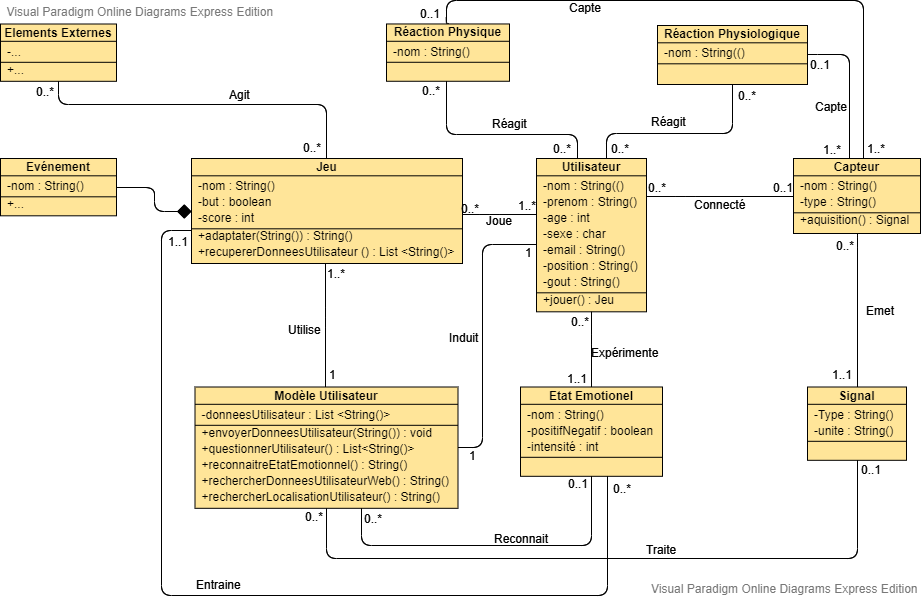
\includegraphics[scale=0.5]{../include/ontologie_stage_cnam-v2-5.png}
			\caption{Ontologie d'un jeu pervasif prenant en compte l'état émotionnel du joueur}
			\label{fig:modele}
		\end{figure}
		Pour chaque classe, il existe une description détaillée en Annexe \ref{ann:detailclasses}
		.\par
		Dans ce modèle, on voit qu'il existe une relaion entre \texttt{Utilisateur}, \texttt{Jeu} et \texttt{Etat Emotionnel} que j'aurais pu représenter par une liaison ternaire.
		Cependadant, j'ai préféré décomposer cette association en trois relations binaires dans un soucis de clareté. 
		Une autre amélioration possible à cette représentation est celle de la relation entre \texttt{Jeu} et \texttt{Modèle Utilisateur}. 
		Avec du recul sur mon travail, je pense qu'il aurait été possible de soit fusionner les deux classes (puisqu'il s'agit d'une relation $1^* - 1$) soit de transformer la classe \texttt{Modèle Utilisateur} en une ou plusieurs autre(s) classe(s).\par
		L'ontologie que je présente dans ce rapport à la Figure \ref{fig:modele} n'est donc pas le résultat définitif.
		En effet, après plusieurs essais et plusieurs versions différentes de l'ontologie, nous avons décidé de changer de point de vue et de revenir, si possible, plus tard à l'ontologie.
	\subsection{Bilan}\label{sec:modelbilan}
		Le bilan que je tire de cet exercice de modélisation est que malgré cet échec d'aboutir à une ontologie livrable, j'ai pu d'une part mieux comprendre la problématique liée au projet et à la conception de modèle.
		Et d'autre part, j'ai pu me rendre compte de l'étendue des difficultés qu'il était possible de rencontrer dans ce genre d'exercice.
		Par exemple, lors de la conception de cette ontologie, je me suis retrouvée à mélanger plusieurs niveaux d'abstraction, ce qui la rendait peu compréhensible et invalide. 
		Je me suis aussi rendu compte qu'il fallait beaucoup de patience et d'entraînement pour concevoir un tel modèle. 
		Aujourd'hui, je comprends mieux les enjeux de tels modèles. 
		A l'avenir je pourrais réaliser des modèles de meilleure qualité grpace à cette expérience.\par
		La réalisation de cette ontologie nous a permis de réorienté notre objectif de recherche vers l'implémentation d'une solution pour la gestion des données générées par les capteurs physiologiques.

\section{Prototypage}\label{sec:prototypage}
	Pour la détection et la reconnaissance de l'état émotionnel, nous utilisons des capteurs physiologiques de contacts.
	Ces capteurs prennent en continue des mesures pour différentes métriques physiologiques telles que la température du corps, le rythme cardiaque, la réponse électrodermale ou encore le rythme respiratoire.
	Ces capteurs génèrent beaucoup de données.
	De plus, il s'agit de données en temps-réel qui doivent être traitées le plus rapidement possible pour reconnaître l'état émotionnel de la personne et ainsi le jeu pourra s'adapter avec un minimum de la latence.
	Une trop grande latence pourrait engendrer un effet de décalage désagréable pour le joueur entre ce qu'il ressent et l'adaptation du jeu.\par
	Dans cette section, nous allons présenter le prototype de notre solution pour gérer les données temps-réel des capteurs.
	Les capteurs physiologiques et les algorithmes de reconnaîssance existent déjà, ils proviennent de précédents travaux effectués au laboratoire.
	Ici nous cherchons à gérer au mieux les données en temps-réel en créant un minimun de latence entre la mesure par le capteur et la reconnaissance de l'état émotionnel.
	\subsection{Technologie utilisée}\label{sec:prototech}
		Pour notre prototype nous avons besoin de gérer efficacement des données continues et en temps-réel.
		Il nous faut donc trouver une technologie capable de traiter efficacement ce genre de données pour les transmettre aux algorithmes de détection et de reconnaissance de l'état émotionnel;
		\subsubsection{Comparaison entre Apache Kafka et RabbitMQ}\label{sec:comparatif}
			Notre choix s'est porté sur les Middleware Orientés Messages (MOM).
			Ces middleware ont pour objectif de transmettre un message d'un utilisateur à un autre.\par
			Nous avons sélectionné deux middlewares libres, simple d'utilisation et avec une communauté active.
			Il s'agit d'Apache Kafka et de RabbitMQ.
			Avan de commencer la synthèse comparative entre ces deux middlewares,  introduisons les points communs entre Apache Kafka et RabbitMQ :
			\begin{itemize}
				\item Middleware orienté message (MOM);
				\item Même ordre de grandeur de message consommable par seconde (un peu + côté Kafka);
				\item Open source;
				\item Modèle d’intégration : Publish / Subscribe (+ point-to-point côté RabbitMQ).
			\end{itemize}
			Apache Kafka et RabbitMQ sont utilisables dans les domaines d'application suivants :
			\begin{itemize}
				\item Collecte d’information pour l'Internet des Objets (IoT);
				\item Transmission de métriques;
				\item Envoi de notifications, de mails, de messages instantanées;
				\item Transmission d’actions utilisateurs;
				\item Actions compte à compte bancaire (transactions).
			\end{itemize}\par
			Maintenant que nous connaissons les points communs entre les deux MOM, nous pouvons en faire une comparaison synthétique.\par
			Dans ce comparatif, nous traitons des principales différences des deux middlewares (Tableau \ref{tab:comparatifinfos}), de leurs architectures (Tableau \ref{tab:comparatifarchi} et Figure \ref{fig:comparatifarchi}), de leurs approches (Tableau \ref{tab:comparatifapp}, des caractéristiques des messages (Tableau \ref{tab:comparatifmess}) et de la préférence d'utilisation de l'un ou de l'autre MOM selon le cas d'usage (Tableau \ref{tab:comparatifpref}).
			\begin{table}[hp]
				\begin{tabular}{|p{7.5cm}|p{7.5cm}|}
					\hline
					\rowcolor{lightgray} RabbitMQ & Kafka\\\hline
					Depuis 2007 & Depuis 2011\\\hline
					Destiné au début : composante primaire dans les messageries SOA ; Maintenant : Flux & Pour le scenario de flux\\\hline
					Structure de données : FIFO; Optimal quand les messages sont livrés rapidement & Structure de données : Log (le consommateur gère l’offset) Possibilité de relire des données, les messages sont conservés selon un temps paramétré\\\hline
					Inclus les protocoles : MQTT, AMQP, STQMP; Facilité pour la communication avec d’autres solutions implémentant AMQP. & Routage simple (clé de routage). Les messages sont sur des « topics » (les consommateurs s’abonnent aux topics voulus)\\\hline
					Mode de délivrance des messages : \textit{at least once} & Modes de délivrance des messages : \textit{at least once} et \textit{exactly once}\\\hline
				\end{tabular}
				\caption{Principales différences / informations générales}
				\label{tab:comparatifinfos}
			\end{table}
			\medskip
			\begin{table}[hp]
				\begin{tabular}{|p{3cm}|p{6cm}|p{6cm}|}
					\hline
					\rowcolor{lightgray} & RabbitMQ & Kafka\\\hline
					Stocakge & Dans une base Mnésia. Quand saturation sur la base Mnésia, stockage sur disque. & Sur disque, dans des fichiers (tailles équiv.), logs. Cluster de servers, dans des topics (Durable). \\\hline
					Routage & Flexible. & Basique.\\\hline
					Structure de\newline données & File FIFO. & Log.\\\hline
				\end{tabular}
				\caption{Architectures}
				\label{tab:comparatifarchi}
			\end{table}
			\medskip
			\begin{figure}[hp]
				\begin{subfigure}{0.6\textwidth}
					\hspace*{-2cm}
					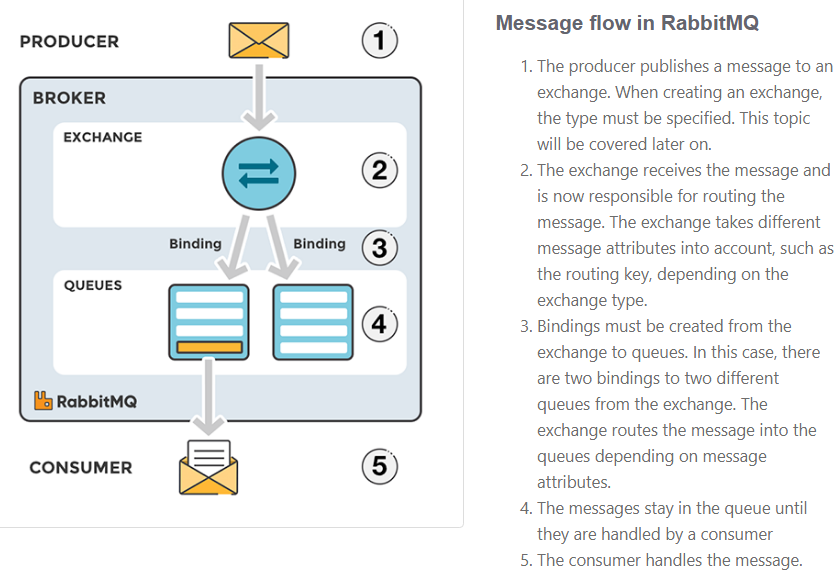
\includegraphics[scale=0.5]{../include/RabbitMQ.PNG}
					\caption{Schéma de l'architecture de RabbitMQ}
					\label{fig:archirabbitmq}
				\end{subfigure}
				\begin{subfigure}{0.5\textwidth}
					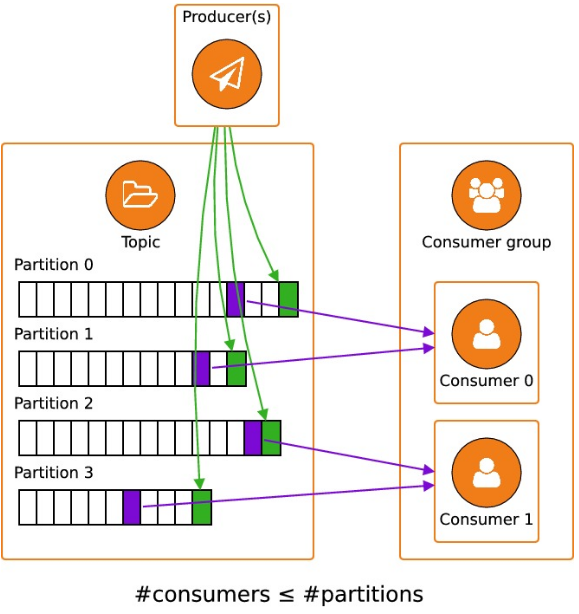
\includegraphics[scale=0.55]{../include/Kafka.PNG}
					\caption{Schéma de l'architecture de Kafka}
				\end{subfigure}
				\caption{Schémas des architectures}
				\label{fig:comparatifarchi}
			\end{figure}
			\medskip
			\begin{table}[hp]
				\begin{tabular}{|p{7.5cm}|p{7.5cm}|}
				\hline
				\rowcolor{lightgray} RabbitMQ & Kafka\\\hline
				\begin{center} \textbf{Approche Push-based :}\end{center} & \begin{center} \textbf{Approche Pull-based :}\end{center}\\\hline
				Distribuer les messages individuellement et rapidement. & Consommateur récupère les lots souhaités à partir d’un offset spécifique ; Mise en commun longue.\\\hline
				\end{tabular}
				\caption{Approches}
				\label{tab:comparatifapp}
			\end{table}
			\medskip
			\begin{table}[hp]
				\begin{tabular}{|p{3cm}|p{6cm}|p{6cm}|}
					\hline
					\rowcolor{lightgray} & RabbitMQ & Kafka\\\hline
					Maintien de l'ordre & Dans une même chaîne (TCP multiplexée) & Dans une même partition\\\hline
					Temps de vie & Jusqu’à que le message soit onsommé (et retour du onsommateur reçu & Délai paramétré (ou si saturation atteinte)\\\hline
					Priorités & Possibilité de définir un degré de priorité des messages & - \\\hline
				\end{tabular}
				\caption{Structure des messages}
				\label{tab:comparatifmess}
			\end{table}
			\medskip
			\begin{table}[hp]
				\begin{tabular}{|p{7.5cm}|p{7.5cm}|}
				\hline
				\rowcolor{lightgray} RabbitMQ & Kafka\\\hline
				Besoin de routages élaborés; Utiliser des protocoles STOMP, MQTT ou AMQP...; Suivi de métriques opérationnelles & Besoin de routages simples ; Conserver (sur temps donné) et relire des messages; Mise à l’échelle; Capture d’évènement induisant un changement d’état (dans une base de données ou autre); Besoins transactionnels ; Traiter les données en parallèle.\\\hline
				\end{tabular}
				\caption{A utiliser de préférence selon le cas d'utilisation}
				\label{tab:comparatifpref}
			\end{table}
			La sitographie sur laquelle je me suis appuyée pour la construction de cette synthèse comparative se trouve en Annexe \ref{ann:kafkarabbitmq}.
		\subsubsection{Positionnement}\label{sec:position}
			Après mes recherches et la rédaction de la synthèse comparative, j'ai décidé d'utiliser Apache Kafka comme Middleware Orienté Message pour le prototypage de notre solution.
			Apache Kafka m'a semblé être plus indiqué dans le traitement des données venant capteurs.
			Ce middleware présente une structue pour les messages en log.
			Ce qui est plus intéressant pour notre cas qu'une structure FIFO (First In, First Out).
			En effet, la structure FIFO nous "oblige" à récupérer et à consommer les messages rapidement dans la queue des messages, alors que le log nous laisse plus de temps.
			Ce qui correspond plus à ce que l'on cherche puisque nous n'allons pas consommer toutes les données pour détecter un état émotionnel, mais seulement à certains moments (lorsqu'un changement significatif sera détecté).
			De plus, les données sont organisées dans des "topics".
			Il est donc possible de récupérer que certaines données en s'abonnant aux topics désirés.
			Cela nous sera très utilie pour de futurs travaux qui impliquerons d'autres capteurs que les capteurs physiologiques pour la reconnaissance des états émotionnels.
	\subsection{Description du prototype}\label{sec:protodesc}
		Dans cette partie, nous allons présenter le prototype de la solution que nous avons implémenté pour répondre aux besoins de gérer des données en temps-réel.\par
		Dans un premier temps nous allons présenter le prototype et son architecture.
		Et dans un second temps, nous montrerons comment nous intégrons le prototype aux travaux déjà menés pour ce projet.\par
		\begin{figure}[t]
			\centering
			\hspace*{-1.7cm}
			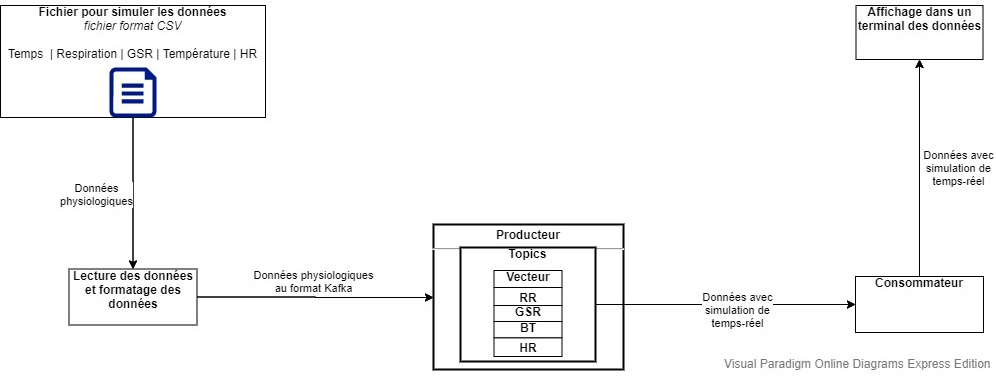
\includegraphics[scale=0.75]{../include/schema-synt-prototype.jpg}
			\caption{Schéma synthétique de l'architecture du prototype}
			\label{fig:archiproto}
		\end{figure}
		La Figure \ref{fig:archiproto} montre l'architecture de notre prototype.
		Pour le moement, nous simulons les données des capteurs.
		Ces données ont été acquisent lors d'une session de jeu vidéo à partir de capteurs physiologiques (capteurs décrits dans la Section \ref{sec:capteurs}.
		Elles ont été enregistrés dans un fichier au format CSV.\par
		Les données sont lus puis envoyées au Producteur.
		Le Producteur ajoute à chaque topic la ou les données qui correspondent.
		Par exemple, les données qui corresponde au Rythme Cardiaque sont envoyés sur le topic "HR" (pour Heart Rate).\par
		Les données peuvent ensuite être consommées par un consommateur qui choisit le topic auquel il s'abonne.
		Les données sont affichés dans un terminal au fur et à mesure qu'elles sont produitent.
		Le consommateur attend toujours de nouvelles données à consommer.
	\subsection{Intégrer le prototype aux travaux déjà menés}\label{sec:travaux}
		Des travaux antérieurs ont été menés pour le projet globale.
		Ces tavaux concernent en particulier la détection et la reoconnaissance d'états émotionnels à partir de capteurs physiologiques.
		Cependant, les algorithmes utilisent des données préalablement acquisent.
		Autrement dit, les mesures physiologiques sont faites et enregistrées dans un fichier excel dans un premier temps.
		Et dans un second temps, les données sont traitées par les algorithmes qui ont été élaborés par des chercheurs du CEDRIC.
		En particulier Viviane GAL dans sa thèse \cite{gal_2019}.
		Il n'y a donc pas de notion de temps-réel dans ces travaux.\par
		C'est pour quoi nous avons mis au point cette solution.
		Nous présentons dans cette partie l'intégration de notre solutions aux travaux qui ont déjà été menés.
		Pour cela, nous allons tout d'abord introduire les capteurs physiologiques qui sont utilisés par les travaux précédents.
		Puis nous allons présenter comment notre solution améliore ces travaux.
		\subsubsection{Capteurs physiologiques utilisés}\label{sec:capteurs}
			Afin que notre prototype transmette les données provenant de capteurs aux algorithmes de reconnaissance des états émotionnels, nous devons nous adapter aux capteurs déjà utilisés par le laboratoire pour les expérimentations passées et futures.
			Nous n'avons pas la possibilité de changer les capteurs, alors c'est à notre solution de s'y adpater.\par
			Les capteurs physiologiques qui sont utilisés dans le projet sont des capteurs de chez TEA Ergo\footnote{\href{https://www.teaergo.com}{https://www.teaergo.com}}.
			Ce sont les capteurs Captiv.
			Ceux que nous possédons permettent la mesure de la fréquence respiratoire, du rythme cardiaque, de la température (à la surface de la peau) et de la réponse électrodermale.
		\subsubsection{Connecteur}
			Pour utiliser notre prototype avec les travaux qui ont déjà été menés pour la recherche des états émotionnels, nous avons besoin d'utiliser un connecteur.
			Ce connecteur va nous permettre de récupérer les données provenant des capteurs pour les formaliser.
			Ainsi elles pourront être utilisées dans Kafka.\par
			Une multitude de connecteurs existent déjà.
			Il s'agit de connecteurs implémentés par Confluent (la plate-forme de Kafka) ou par la communauté.
			Sur le Confluent Hub\footnote{\href{https://www.confluent.io/hub/kafka-connectors-33}{https://www.confluent.io/hub/kafka-connectors-33}}, nous avons pu rechercher le connecteur qui convenait le mieux pour notre cas.
			Sur ce hub, 165 connecteurs sont proposés.
			Certains connecteurs permette de récupérer des données sources, d'autres permettent d'évacuer les données vers des structures externes et d'autres permettent de transformer les données.
			Certains connecteurs permettent même de faire deux ou trois de ces types d'actions.
			Nous nous sommes intéressés ici aux connecteurs sources.
			Nous allons vous présenter les différents connecteurs sources que nous avons pu répertoriés.\par
			Pour notre recherche, nous avons appliqués les filtres suivants : \newline
			Plugin type $=$ "Source" et License $=$ "Free".\newline
			Comme indiqué plus haut, nous recherchons un connecteur source.
			De plus, nous avons préféré nous restreindre aux licences libres pour avoir au moins une vue sur le code qui est utilisé.\par
			La recherche nous a donné 38 connecteurs.
			Nous avons trié ces connecteurs en deux sous-parties :
			\begin{itemize}
				\item Les connecteurs potentiels : Les connecteurs qui peuvent servir pour notre cas, c'est-à-dire qu'ils peuvnet faire de l’ingestion de données en temps-réel;
				\item Les connecteurs non-retenus : Les connecteurs jugés trop éloignés de notre cas d’usage pour des raisons diverses.
				% Ils sont soit orienté sbases de données relationnelles, soit orientés fichiers systèmes, soit générateurs de données factices, etc.
			\end{itemize}
			Voici tableaux reprenant chaque connecteur et une petite description.\par
			\textbf{1. Les connecteurs potentiels}\par
			Ces connecteurs vont permettre de récupérer des données en temps-réel. 
			Comme nos capteurs diffusent en permanence, nous avons besoin d’un Connecteur capable de transférer des données en temps-réel depuis les capteurs vers Kafka.
			Le tableau \ref{tab:connecteurspotentiels} répertorie ces connecteurs.
			\begin{table}[h]
				\begin{tabular}{|p{7.5cm}|p{7.5cm}|}
					\hline
					\rowcolor{lightgray} Connecteur & Description\\\hline
					Diffusion® Kafka Connector & Permettre aux clients web, mobile et IoT de consommer et envoyer des données temps-réel et orientées-événement\\\hline
					Kafka Connect Shell & Ingère la sortie d’une commande passé dans le shell vers Kafka (peut être utilisé avec un algorithme déjà implémentés de travaux antérieurs) \\\hline
				\end{tabular}
				\caption{Les connecteurs potentiels}
				\label{tab:connecteurspotentiels}
			\end{table}\par
			\textbf{2. Les connecteurs non-retenus}\par
			Ces connecteurs peuvnet être écartés de nos recherches. 
			Ces plug-in sont soit trop spécifiques, soit orientés bases de données relationnelles, soit pour des fichiers systèmes, soit pour créer des données factices, etc.
			Le tableau suivant repertorie ces connecteurs.
			\begin{longtable}{|p{7.5cm}|p{7.5cm}|}
				\hline
				\rowcolor{lightgray} Connecteur & Description\\\hline
				\endhead
				Kafka Connect JDBC & Pour les bases de données relationnelles JDBC\\\hline
				Kafka Connect JDBC with Flatten Feature & Extension de Kafka Connect JDBC\\\hline
				Debezium MySQL CDC Connector & Surveillance et enregistrement des changements pour MySQL server\\\hline
				Debezium PosgreSQL CDC Connector & Surveillance et enregistrement des changments pour les bases de données PostgreSQL\\\hline
				Debezium SQL server CDC Connector & Surveillance et enregistrement des changements pour des serveurs SQL\\\hline
				MongoDB Connector for Apache Kafka & Récupérer des données depuis une base de données MongoDB.\\\hline
				Debezium MongoDB CDC Connector & Surveillance des ensemble de réplicas MongoBD\\\hline
				Kafka Connect Spooldir & Pour des fichiers délimités de fichiers systèmes\\\hline
				Couchbase DB Connector & Transférer des données depuis et vers Couchbase server\\\hline
				Kafka Connect Crux & Transférer des données depuis et vers les nœuds Crux\\\hline
				Kafka Connect Venafi & Se connecter à Venafi Platform via HTTP et récupérer des événements logs depuis Kafka. Filtrage, transformation, traitement possible.\\\hline
				Kinetica DB Connector & Pour Kinetica, base de données distribuée en mémoire accélérée par GPU. Ingèrer, analyser et visualiser en même temps\\\hline
				SAP Hana Connector & Pour les systèmes SAP\\\hline
				Databricks Connector for Apache Kafka & Se connecter à une base de données Databricks et d'envoyer les données vers Kafka.\\\hline
				Levy Xenon Connector & Pour fort I/O et bigData\\\hline
				CockroachDB Change Data Capture & Fonctionnalité de capture de changement de ligne dans la BD\\\hline
				Hazelcast Jet Kafka Connector & Offre un producer et un consumer pour transférer des données entre Kafka et Hazelcast\\\hline
				StreamSets Data Collector & Simplifier la construction, l’éxecution et les opérations pour les flots de données\\\hline
				Kafka Connect IRC & Connecteur source pour IRC\\\hline
				Kafka Connect HTTP & Pour les APIs JSON/http\\\hline
				Kafka Connect Sound & Lire des données de microphone et envoyer des données pour sortie audio\\\hline
				Kafka Connect Reddit & Récupérer des posts et des commentaires en temps-réel via Reddit\\\hline
				Kafka Connect FileSystem & Lire différents formats de fichiers de différents types de fichiers système\\\hline
				Kafka Connect Common Transfomations & Transformation de données de fichiers.\\\hline
				Kafka connect-pulsar & Permet de répliquer des données de Apache Pulsar vers Apache Kafka\\\hline
				Kafka Connect Maxmind Transformation & Pour ajouter des données GeoIP aux données Kafka\\\hline
				Kafka Connect Twitter & Flux de données Twiitter vers Kafka\\\hline
				Kafka Connect Email & POM parent pour les projets Kafka Connect\\\hline
				Kafka Connect Simulator & Générer des données de test\\\hline
				Kafka Connect RSS Source & Récupérer des données de flux RSS et Atom\\\hline
				Kafka Connect Flume Avro & Envoyer des données depuis Apache Flume\\\hline
				Voluble & Générateur de données factices\\\hline
				Apache Connect IoT Hub & Pour Azur IoT Hub\\\hline
				Kafka Connect Zeebe	& Enregistrements de workflow BPMN vers kafka\\\hline
				Kafka Connect File Pulse & Parse, transfomer et charger les données  depuis un fichier système local vers Kafka\\\hline
				\caption{Les connecteurs non-retenus}
				\label{tab:connecteursnon}
			\end{longtable}\par
			\textbf{3. Positionnement}\par
			Parmis les deux connecteurs que nous avons retenus, nous avons décidé d'utiliser le connecteur \texttt{Kafka Connect Shell}\footnote{\href{https://www.confluent.io/hub/thomaskwscott/kafka-connect-shell-source}{https://www.confluent.io/hub/thomaskwscott/kafka-connect-shell-source}}.
			Dans l'optique d'être plus rapide dans nos tests, ce connecteur nous semble être le meilleur choix.
			Nous allons l'utiliser avec un algorithme déjà existant provenant de travaux antérieurs qui affiche les données des capteurs dans un terminal.
			Avec le connecteur Kafka Connect Shell, nous seront capable de lire les données affichées sur le terminal et de les transmettre au Producteur Kafka.
		\subsubsection{Schéma de l'intégration du prototypes aux travaux déjà menés}\label{sec:schematravaux}
			\begin{figure}
				\centering
				\vspace*{-1cm}
				\rotatebox{90}{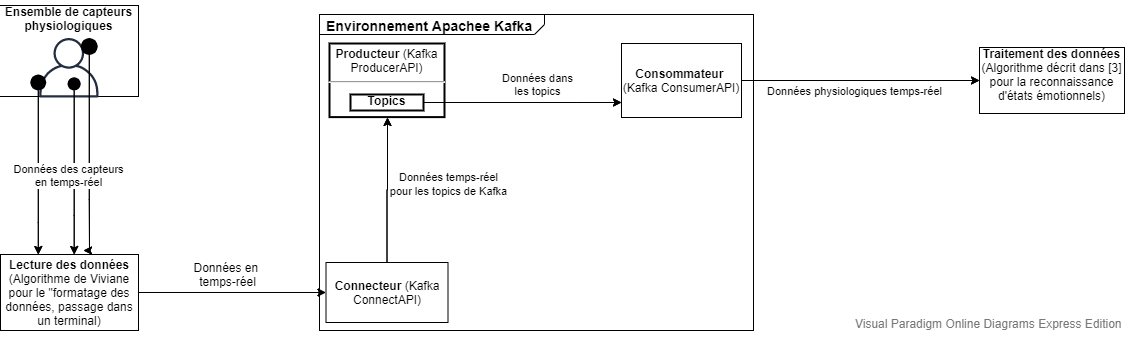
\includegraphics[scale=0.75]{../include/schema-global.jpg}}
				\caption{Schéma de l'architecture du prototype intégré au projet}
				\label{fig:archiglobale}
			\end{figure}
			L'architecture présentée à la Figure \ref{fig:archiglobale} nous permet de voir l'intégration de notre solution aux travaux menés précédemment.
			Comme il existe déjà un algorithme qui permet de lire les données des capteurs et de les afficher sur un terminal, nous l'utilisions.
			Le Connecteur que nous utilisons permet de récupérer des données sur un terminal et de les transmettre au Producteur sous la bonne forme pour être envoyées dans les topics.
			Les topics sont ensuite consommés par les algorithmes de reconnaissance de l'état émotionnel.
	\subsection{Validation}\label{sec:validation}
		L'objectif que nous avions pour ce prototype était de pouvoir récupérer des données provenant de capteurs et de les envoyés vers les algorithmes de détection et de reconnaissance d'états émotionnels\par
		Dans ce rapport, nous prposons une solutiion que nous avons implémenté.
		Elle est actuellement testée avec un fichier au format .CSV contenant les données de quatre capteurs physiologiques : la fréquence respiratoire, la réponse électrodermale, la température corporelle et la fréquence cardiaque.
		Chaque ligne de ce fichier est envoyée dans les topics avec 30 milisecondes (ms) d'écart.
		Ces 30ms correspondent au temps moyen d'acquisition entre deux données.
		Cela nous donne une impression de temps-réel.
		Les données sont ensuite lues par un consommateur qui les affiche au fur et à mesure dans un terminal.\par
		Du point de vue de l'objectif que nous avions fixé pour ce prototype, nous pouvons dire que cette implémentation correspond à ce que nous voulions réaliser.
		Les données sont bien lues et renvoyées pour être analyses.
			
\section{Conclusion}\label{sec:conclusion}
	L'objectif principal de ce projet est réaliser un jeu pervasif adaptable dynamiquement aux états émotionnels du joueur.
	Pour ce faire, il nous utilisons des capteurs physiologiques qui génèrent des données analysées par des algorithmes pour la détection et la reconnaissance e l'état émotionnel.
	Une fois l'état émotionnel reconnu, le jeu peut alors proposer au joueur l'événement le plus adéquat pour garantir le meilleur divertissement possible aux joueurs.
	Avec cet objectif en tête, nous avons chercher un moyen efficace de gérer les données fournies en continu par les capteurs.\par
	Dans ce rapport, nous avons présenté plusieurs travaux qui ont été mené tout au long de ce travail.
	Cette contribution a été avant tout l'occasion de d'affiner les besoins pour un jeu pervasif adaptable aux états émotionnels du joueur.
	En premier lieu, nous avons fait l'état de l'art des méthodes permettant la détection et la reconnaissance d'états émotionnels dans le domaines des jeux.
	Puis, nous avons aborder la notion d'expérience utilisateur et l'expérimentation que nous avons mené lors d'un escape game.
	Ensuite, nous avons présenté notre première tentative de solution sous la forme d'un modèle conceptuel pour représenter l'adaptation d'un jeu pervasif aux états émotionnel d'un joueur.
	Enfin, nous avons présenté le prototype de notre solution pour la gestion des données provenant de capteurs physiologiques pour que ces données soient utilisées avec des algorithmes déjà existants.\par
	Cette dernière solution que nous avons détaillée dans ce rapport a été implémenté permet de lire et d'envoyer en temps-réel (avec le minimum de latence possible) les données sur des topics.
	Durant ce travail de près de six mois, j'ai beaucoup appris.
	J'ai appris une certaine rigueur.
	Une rigueur tout d'abord dans mes lectures.
	Au fil des lectures que j'ai faites, j'ai noté de plus en plus de détails dans mes résumés pour éviter d'avoir à y revenir trop souvent,
	Une rigueur au niveau de la rédaction.
	J'ai appris a être très rigoureuse sur la forme de mes rédactions.\par
	Ce travail a été l'occasion d'affiner les contour du projet.
	Plusieurs perspectives sont a envisager.
	Tout d'abord il faudrait mettre à l'épreuve notre prototype directement avec nos capteurs.
	Si les tests avec les capteurs sont satisfaisants, alors il sera possible de passer à l'étape de la conception d'algorithmes pour l'adaptation selon l'état émotionnel courant du joueur.
	Il faudra par la suite développer d'autres aspects lié au jeu lui-même.
	Comme par exemple la jouabilité ou le game design.
	Un objectif de ce projet est d'utiliser ce jeu à d'autres domaines d'applications que celui du divertissement.
	On peut imaginer utiliser ce jeu pour enseigner des émotions par exemple.
	Il faudra donc garder un aspect très générique de ce jeu.


\newpage
\renewcommand{\contentsname}{Annexes}\appendix
\section{Adaptation d’un jeu pervasif particularisé basée sur l'état émotionnel et sur les caractéristiques du joueur – État de l’art}\label{ann:eda}
	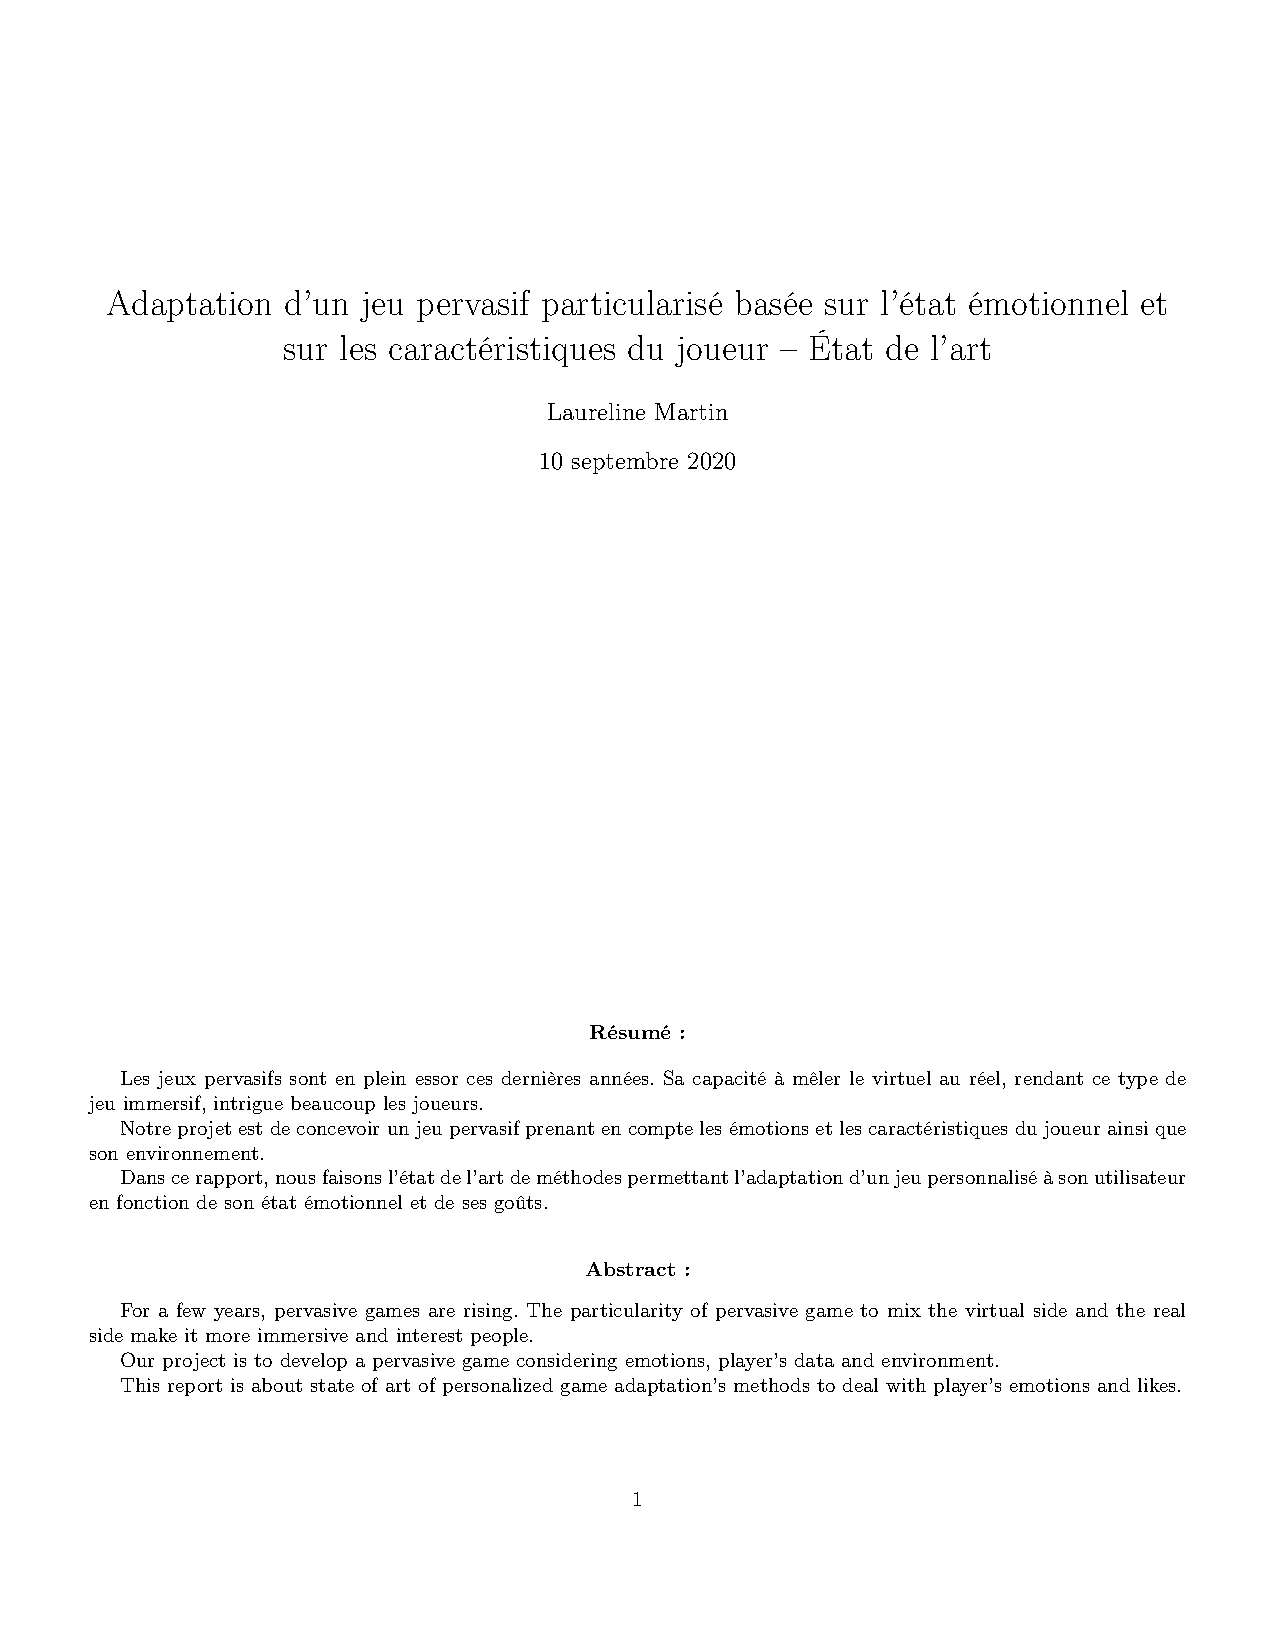
\includepdf[pages=-]{../include/eda.pdf}

\section{Description détaillée des classes de l'ontologie}\label{ann:detailclasses}
	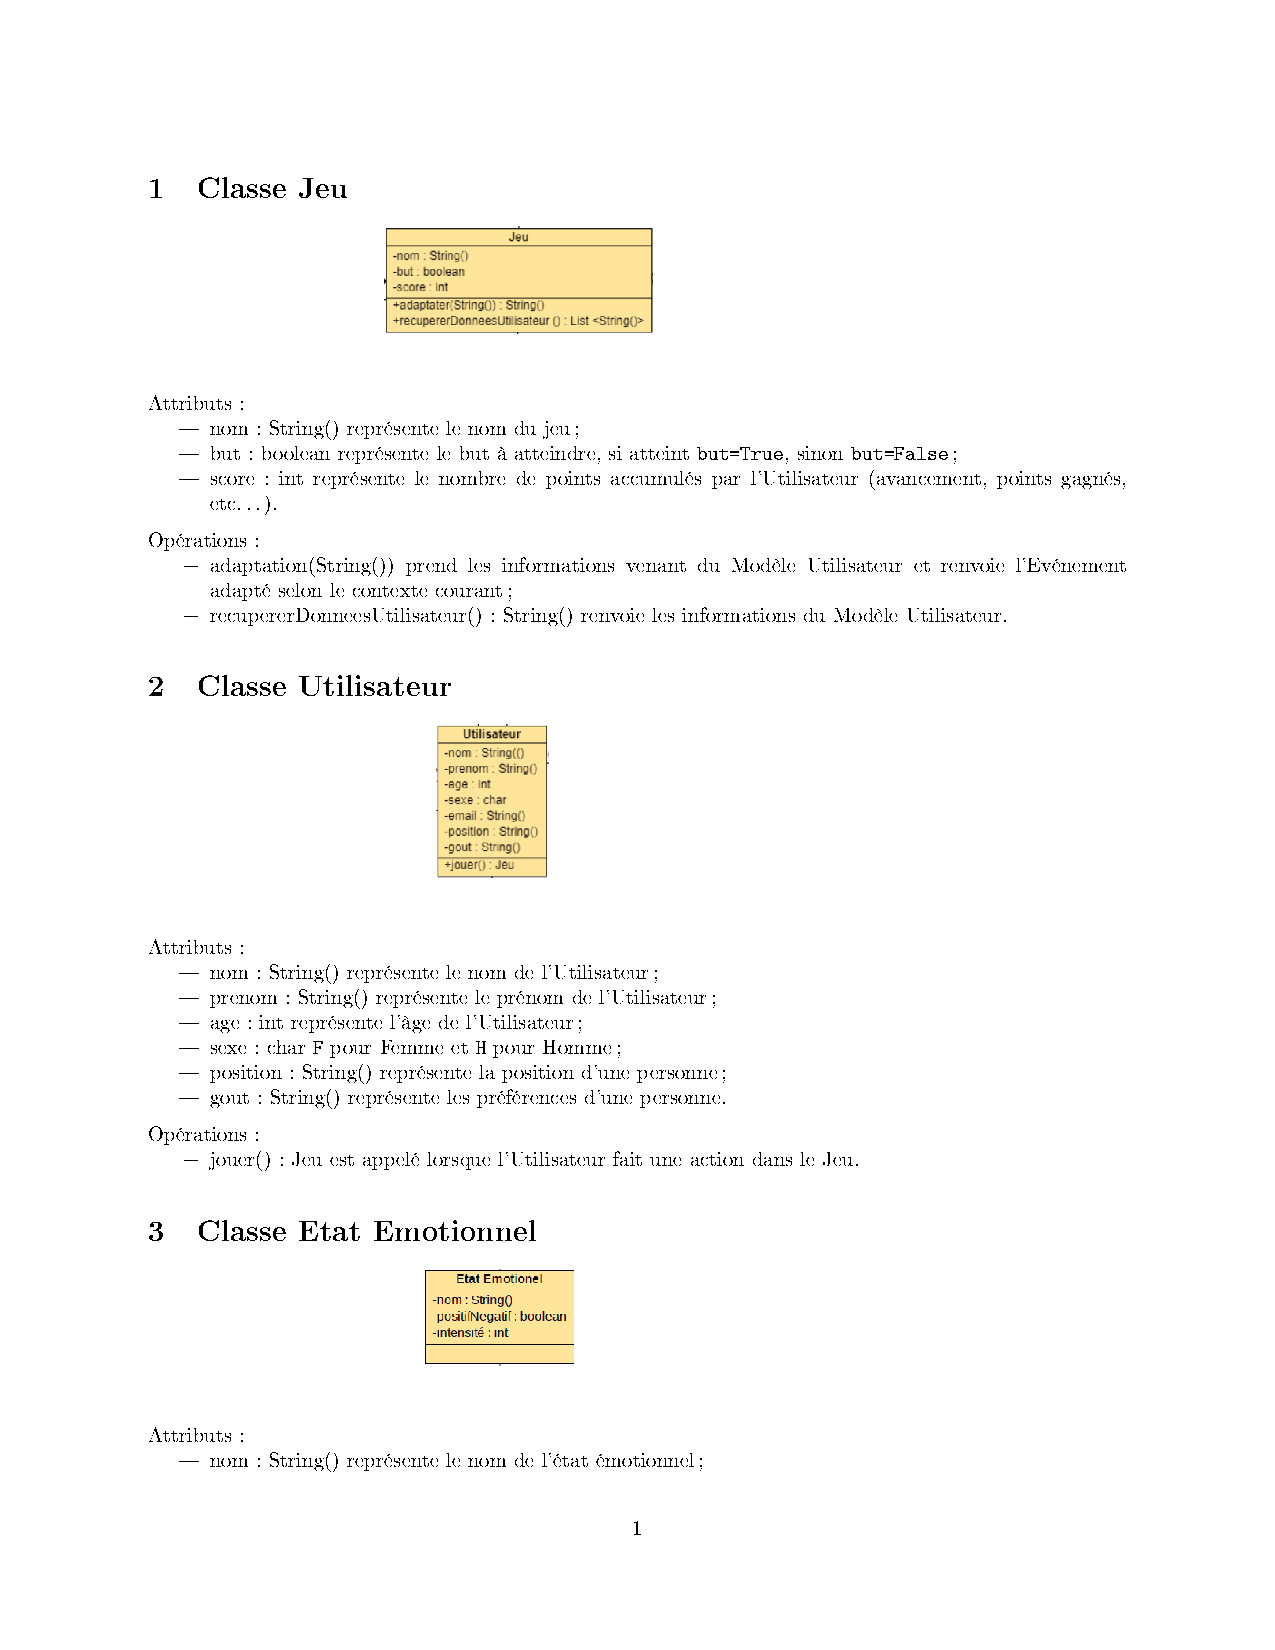
\includepdf[pages=-]{../include/descriptionClassesOntologie.pdf}

\section{Sitographie pour la construction de la synthèse comparative entre Kafka et RabbitMQ}\label{ann:kafkarabbitmq}
	\hspace*{-0.5cm}\href{https://www.upsolver.com/blog/kafka-versus-rabbitmq-architecture-performance-use-
	case}{https://www.upsolver.com/blog/kafka-versus-rabbitmq-architecture-performance-use-
	case} \textit{[en]} \medskip\newline
	\href{https://blog.ippon.fr/2018/03/27/comparatif-rabbitmq-kafka/}{https://blog.ippon.fr/2018/03/27/comparatif-rabbitmq-kafka/} \textit{[fr]}\medskip\newline
	\href{https://www.cloudamqp.com/blog/2015-05-18-part1-rabbitmq-for-beginners-what-is-rabbitmq.htm}{https://www.cloudamqp.com/blog/2015-05-18-part1-rabbitmq-for-beginners-what-is-rabbitmq.htm} \textit{[en]}\medskip\newline
	\href{https://openclassrooms.com/fr/courses/4451251-gerez-des-flux-de-donnees-temps-reel/4451521-metamorphosez-vos-applications-temps-reel-avec-kafka}{https://openclassrooms.com/fr/courses/4451251-gerez-des-flux-de-donnees-temps-reel/4451521-metamorphosez-vos-applications-temps-reel-avec-kafka} \textit{[en]}
	%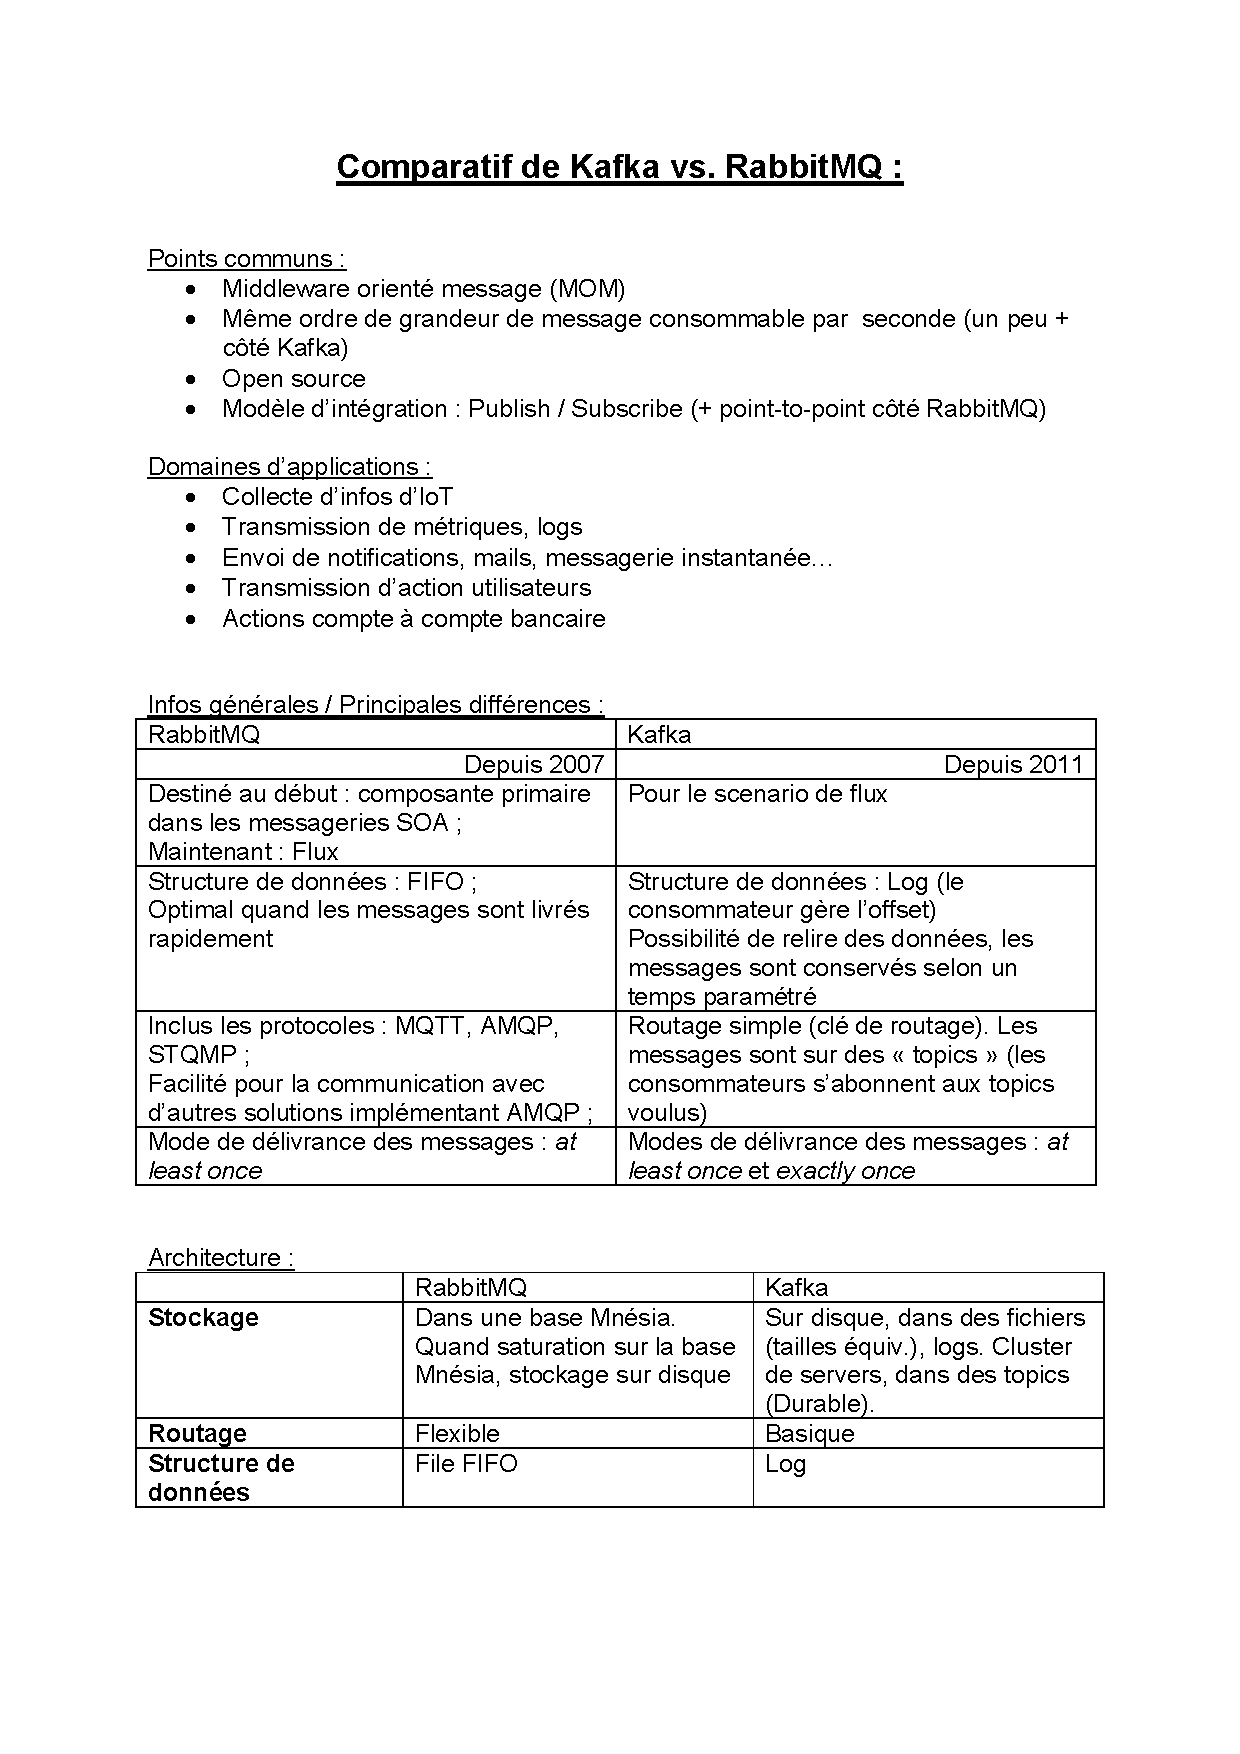
\includepdf[pages=-]{../include/comparatifKafkaVSRabbitMQ.pdf}	

\section{Offre de stage}\label{app:annexe1}
	\textbf{Elaboration du modèle conceptuel des jeux pervasifs adaptables avec la prise en compte des états émotionnels des joueurs}\par
	\medskip
	\textbf{Contexte :}\newline
	Le champ des jeux affectifs est nouveau. Il s’appuie sur l’intégration de nouveaux moyens à développer dans les jeux afin d’adaptabilité. [1] et [2] présentent une méthodologie unifiée pour la conception des jeux affectifs utilisant le plus tôt possible le mécanisme de boucle émotionnelle. Ils repèrent des variations à l’aide de mesures physiologiques et appliquent un modèle issu d’un ensemble construit considéré comme en relation avec les émotions. Leur étude montre combien la dimension émotionnelle de l’utilisateur est importante mais difficile à gérer.\newline
	Le profil du joueur, y compris ses émotions, impacte la conception des jeux. Afin de proposer une meilleure expérience aux joueurs et de proposer un jeu particularisé, le jeu doit être adaptable en fonction du contexte global du joueur. Nous sommes dans une approche holistique qui combine à la fois l’individu et ses émotions, et, les influences de l’entourage qui va du bâtiment lui-même à l’atmosphère que dégage le lieu. Très peu de travaux ont été faits pour la conception et le développement des jeux adaptables dynamiquement. [3] formalise le concept des jeux appliqués aux visites de musées. Ce travail modélise le jeu de visite et propose un processus d’équilibrage entre la dimension ludique et la dimension non ludique (la visite) de ce type de jeux. [3] propose des patrons de mission qui servent d’éléments réutilisables lors de la conception des jeux, mais qui ne couvrent qu’une partie du processus de conception.\par
	\textbf{Sujet :}\newline
	Il s’agit dans ce stage d’élaborer un modèle conceptuel du jeu pervasif adaptable basé sur les émotions. Ce modèle, éventuellement réalisé sous forme d’une ontologie, doit couvrir toute la variété des facteurs qui impactent le jeu tels que le profil de l’utilisateur et ses données physiologiques exprimant son état émotionnel. Cette ontologie doit être construite de façon à ce qu’elle soit adaptée à la démarche situationnelle nécessaire pour la composition dynamique du jeu.

\bibliographystyle{abbrv}
\bibliography{../include/biblio}
\end{document}